\documentclass[]{article}

\usepackage[T1]{fontenc}
\usepackage[utf8]{inputenc}
\usepackage{amsthm, amsmath, amsfonts}
\usepackage{blkarray}
\usepackage{bigstrut}
\usepackage{graphicx}
\usepackage[left=2.5cm, right=2.5cm]{geometry}

\newcommand{\avaliacao}{2}
\newcommand{\disciplina}{Probabilidade e Estatística}
\newcommand{\semestre}{2024/1}


\theoremstyle{definition}
\newtheorem{ex}{Exercício}

\renewcommand{\SS}{\mathcal{S}}

\begin{document}
\thispagestyle{empty}
\begin{center}
\Large{Prova final de \disciplina\ - \semestre}

\large{Prof. Dr. Alessandro José Queiroz Sarnaglia}
\end{center}

\begin{ex}
Um sistema tem 4 componentes idênticos. A probabilidade de um componente não apresentar defeito em um
dia é de 0,7. Assuma independência dos componentes.
\begin{enumerate}
	\item Encontre a probabilidade de pelo menos um componente apresentar defeito; \textbf{Resp.:} 0,7599
	\item Encontre a probabilidade de pelo menos um componente não apresentar defeito; \textbf{Resp.:} 0,9919
	\item Encontre a probabilidade de exatamente um componente apresentar defeito. \textbf{Resp.:} 0,4116
\end{enumerate}
\end{ex}

\begin{ex}
Determinado evento ocorre em um ponto $(X,Y)$ na região ilustrada abaixo.
\begin{center}
	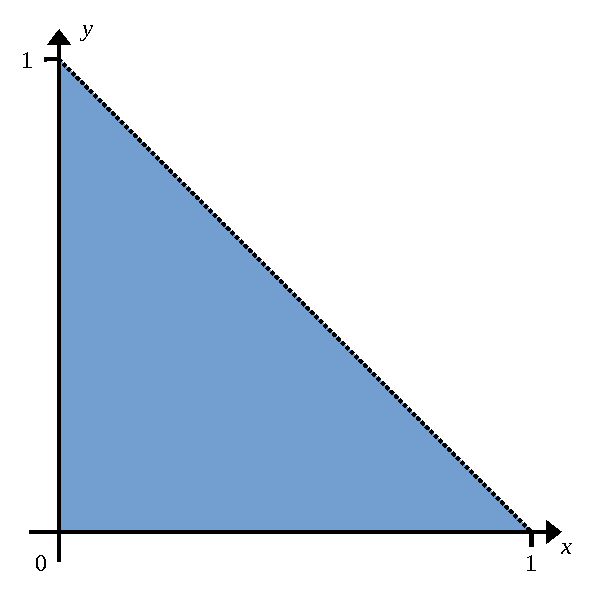
\includegraphics[width=0.4\linewidth]{figura_pf}
\end{center}
Suponha que nenhum ponto é privilegiado para a ocorrência do evento.
\begin{enumerate}
	\item Encontre as fdp's marginais de $X$ e $Y$. \textbf{Resp.:} $f_X(x) = 2(1-x)$, $0\leq x \leq 1$, e $f_Y(y) = 2(1-y)$, $0\leq y \leq 1$.
	\item Encontre $\text{Cov}(X,Y)$. \textbf{Resp.:} $\text{Cov}(X,Y) = -\frac{1}{36} \approx -0\text{,}0278$.
\end{enumerate}
\end{ex}

\begin{ex}
Seja $X_1, \ldots, X_n$ amostra aleatória de uma população $X$ com fdp
$$
f_X(x;\alpha) = \frac{1}{\alpha}x^{\frac{1-\alpha}{\alpha}}, \ \ \ 0<x<1.
$$
\begin{enumerate}
	\item Encontre o Estimador de Máxima Verossimilhança (EMV) $\hat\alpha$ do parâmetro $\alpha$; \textbf{Resp.:} $\hat\alpha = -\frac{\sum_i\log(X_i)}{n}$.
	\item Encontre o vício $B(\hat\alpha) = E(\hat\alpha) - \alpha$ do EMV $\hat\alpha$. \underline{\textit{Dica:}} \textit{É possível mostrar que $E[\log(X_i)] = -\alpha$}; \textbf{Resp.:} Temos $E(\hat\alpha) = -\frac{\sum_iE[\log(X_i)]}{n} = -\frac{n(-\alpha)}{n} = \alpha$. Logo, $B(\hat\alpha) = \alpha-\alpha = 0$.
	\item Utilize as $n=10$ observações e seus logaritmos a seguir para estimar $\alpha$:
	\begin{center}
		\begin{tabular}{c|cccccccccc}
			\hline
			$x_i$& 0,70& 0,34& 0,52& 0,45& 0,52& 0,62& 0,60& 0,83& 0,37& 0,74\\
			\hline
			$\log(x_i)$& -0,36& -1,08& -0,65& -0,80& -0,65& -0,48& -0,51& -0,19& -0,99& -0,30\\
			\hline
		\end{tabular}
	\end{center}
	\textbf{Resp.:} $\hat\beta = 0\text{,}601$.
\end{enumerate}
\end{ex}
\end{document}
